	\section{PAN Einrichtung}
		\label{sec:pan}
		Wird im Hauptmenü noch nicht die richtige IP-Adresse angezeigt, müssen zuerst die PAN\footnote{PAN = Personal Area Network}-Einstellungen korrigiert werden.
		
		\begin{enumerate}	
			\begin{minipage}{.45\textwidth}
				\item Dazu musst du zuerst in das \textbf{PAN-Menü} des Roboters navigieren. Wechsle mit den Links-/Rechts-Tasten bis du den Menüpunkt \textbf{PAN} siehst und betätige die \textbf{Auswahltaste}.
			\end{minipage}
			\hfill
			\begin{minipage}{.45\textwidth}
				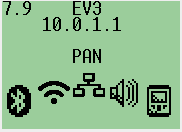
\includegraphics[width=.8\textwidth]{img/ev3_pan.png}
			\end{minipage}
			
			\item Nun navigierst du durch das Menü des Roboters wie auf den Bildern zu sehen und bestätigst jeweils mit der Auswahltaste: \textbf{USB-Client - Address - Advanced}
			
			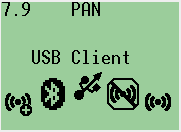
\includegraphics[width=.3\textwidth]{img/ev3_pan_usb.png}
			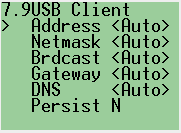
\includegraphics[width=.3\textwidth]{img/ev3_pan_usb_address.png}		
			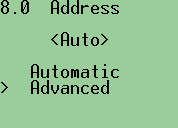
\includegraphics[width=.3\textwidth]{img/ev3_pan_usb_advanced.png}
			
			Nun musst du die IP Adresse 192.168.42.253 einstellen. Dazu navigierst du mit den rechts-/links-Tasten zu den einzelnen Ziffern und änderst deren Wert mit den oben-/unten-Tasten. Orientiere dich an den Bildern! Am Ende bestätigst du wieder mit der Enter-Taste. 
			
			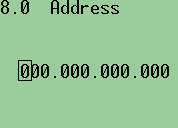
\includegraphics[width=.3\textwidth]{img/ev3_pan_usb_setip1.png}
			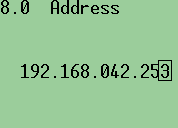
\includegraphics[width=.3\textwidth]{img/ev3_pan_usb_setip2.png}
			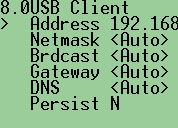
\includegraphics[width=.3\textwidth]{img/ev3_pan_usb_isset.png}
			
			\begin{minipage}{.6\textwidth}
				\item Mit der \textbf{Zurück}-Taste kommst du wieder in das Hauptmenü und die Einstellungen werden übernommen.
			\end{minipage}
			\hfill
			\begin{minipage}{.3\textwidth}
				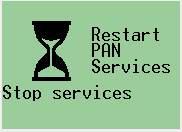
\includegraphics[width=\textwidth]{img/ev3_pan_usb_restart.png}
			\end{minipage}
			%		\\Nun kannst du wieder zu Punkt 3 auf Seite \pageref{sec:afterpan} wechseln.
		\end{enumerate}
		
		\section{Troubleshooting}
		\subsection{Installation über WLAN funktioniert nicht}
		Im Message-Server über \bfcode{File->Connected Devices }schauen ob alle Smartphones in der Liste auftauchen und der ADB-state auf \bfcode{connected} steht. 
		Ist dies nicht der Fall, tippe in der App auf \bfcode{TRENNEN} und stelle die Verbindung danach erneut her.
		Falls das nicht klappt, kontaktiere einen Betreuer. 
		Falls das Installieren per WLAN gar nicht mehr funktioniert, kann jederzeit eine USB-Verbindung zwischen Smartphone und PC hergestellt werden und darüber die App installiert werden.
		
		
		
		\section{Sensorbelegung}
		
		Tabelle	\ref{tab:sensors} zeigt die standardmäßige Sensorbelegung, wie sie in der App unter ``Mein Roboter'' definiert sein muss.\\
			
	
		\begin{table}[h]
			\begin{center}
				\begin{tabular}{r|l|l}						
					\textbf{Anschluss} & \textbf{Sensortyp} & \textbf{Modus} \\ \hline
					1 & Farbe & ColorID \\ 
					2 & Ultraschall & Distance \\ 
					3 & Gyroskop & Angle \\ 
					4 & Farbe & ColorID \\ 
				\end{tabular}
				\caption{Sensorbelegung}
				\label{tab:sensors}
			\end{center}
		\end{table}
	
		Tabelle \ref{tab:motors} zeigt den standardmäßigen Motoranschluss, wie er in der App unter ``Mein Roboter'' definiert sein muss.\\
		
		\begin{table}[h]
			\begin{center}
				\begin{tabular}{r|l}						
					\textbf{Anschluss} & \textbf{Motor} \\ \hline
					A & Large Regulated Motor \\ 
					B & - \\ 
					C & - \\ 
					D & Large Regulated Motor \\ 
				\end{tabular}
			\end{center}
			\caption{Motorbelegung}
			\label{tab:motors}
			\end{table}
	\end{document}